\chapter{Experiments in 3D mapping} \label{experiments_3d_mapping}

\section{Overview}

In this chapter, we transition to using various 3D mapping solutions for real-time mapping on the Turtlebot4, running ROS2. This involved extensive testing of RTAB-Map~\cite{RTAB_Map_docs} with the OAK-D camera and Nvidia's nvblox~\cite{nvblox_docs} to assess their effectiveness and identify any limitations, particularly in terms of speed and orientation tracking.

Since the Turtlebot4 is running ROS2, I needed to find a tool that can do the mapping and runs on the said framework. We have experimented with RTAB-Map (Real-Time Appearance-Based Mapping) and nvblox.


\section{RTAB-Map using OAK-D} \label{experiments_rtab_map}
First, I tried out RTAB-Map with the OAK-D camera. It is already implemented in ROS2 and it can be launched with the following command:
\FloatBarrier
\begin{lstlisting}[language=bash,frame=single,float=!ht]
$ ros2 launch depthai_ros_driver rtabmap.launch.py
\end{lstlisting}

The launched tool's UI can be seen on Figure \ref{fig:rtabmap_ros}. The top left panel shows the last keyframe captured by the camera, under it we can see the actual image recorded by it. On the right, we can inspect the built map:

\begin{figure}[htbp]
	\centering
	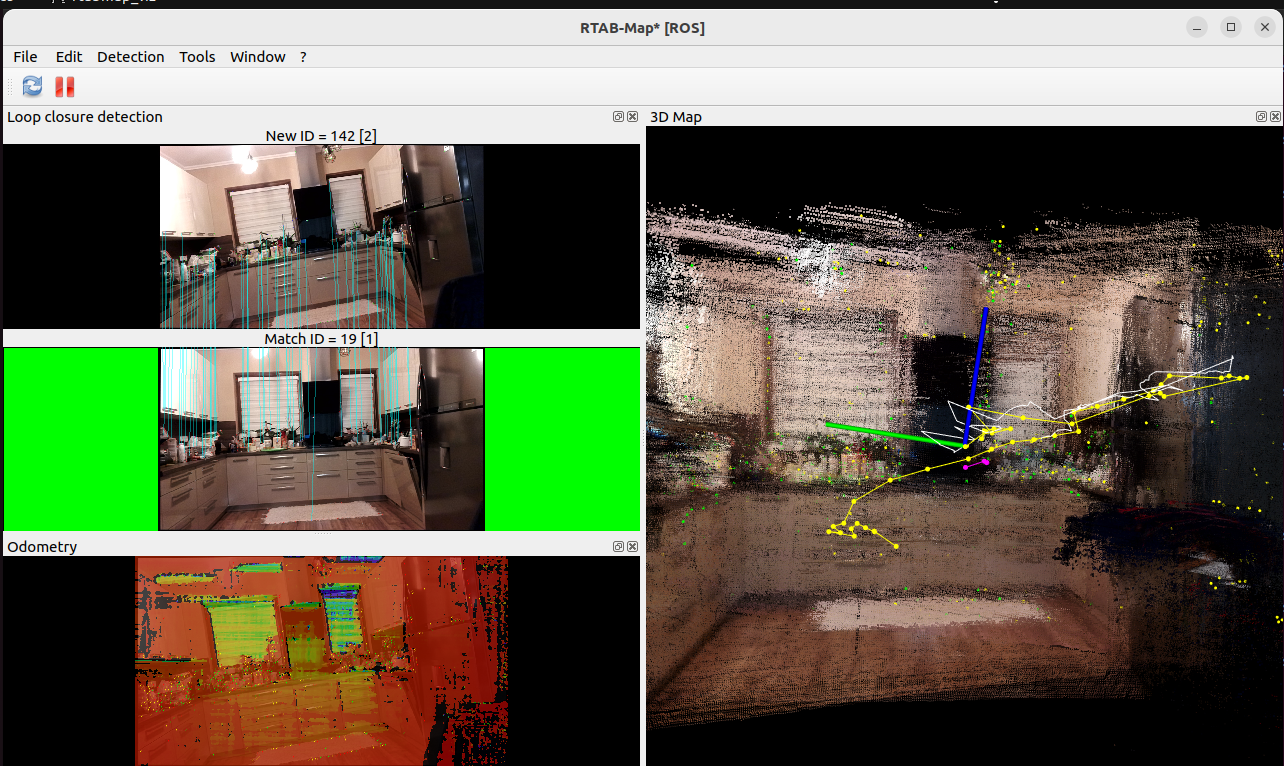
\includegraphics[width=150mm, keepaspectratio]{figures/rtabmap_ros.png}
	\caption{RTAB-Map ROS2}
	\label{fig:rtabmap_ros}
\end{figure}

When the device loses its orientation, it shows the last known position on the bottom left panel. When this happens the mapping stops and we have to navigate back to the exact same position where we lost track to get back on it and continue with the mapping. This is a huge downside of the application because this can happen quite a lot (especially in environments with poor lighting). Furthermore, we sometimes had to restart the entire mapping process because, although we returned the camera to the last known position, RTAB-Map could not recognize it. Another disadvantage of the tool is its speed; the camera's image lags significantly.

For the appropriate usage of RTAB-Map we had to modify its launch files. Our goal was to start the camera on the robot (because it is attached to it), then publish the images and IMU data onto a ROS topic which can be processed by the notebook on top.

When we start the \verb|rtabmap.launch.py| launch file inside the \verb|depthai_ros_driver| package it automatically starts the camera's node in addition to the RTAB-Map node. It was not ideal for us since the camera node should run on the robot and the RTAB-Map (which requires more computation resources) on the notebook. Our solution was to create a new launch file (which can be examined at \ref{rtabmap_custom_launch_file}) based on \verb|rtabmap.launch.py| which starts everything but the camera node. With the help of this we can launch RTAB-Map on the notebook without the camera. The camera can be started on the robot with the basic \verb|camera.launch.py| launch file from the \verb|depthai_ros_driver| package. A mapping made with this approach can be seen on Figure~\ref{fig:rtabmap_nokia}.

To summarize our experiments, due to the lag and loss of orientation, it was problematic to create a map even in a small room (seen on Figure~\ref{fig:rtabmap_nokia}, it can be seen that a lot of irrelevant points are added to the map). This issue is more severe on the actual robot, which can turn at high angular speeds. It always lost track, and navigating back to the last known position was time-consuming and only moderately successful.

\begin{figure}[H]
	\centering
	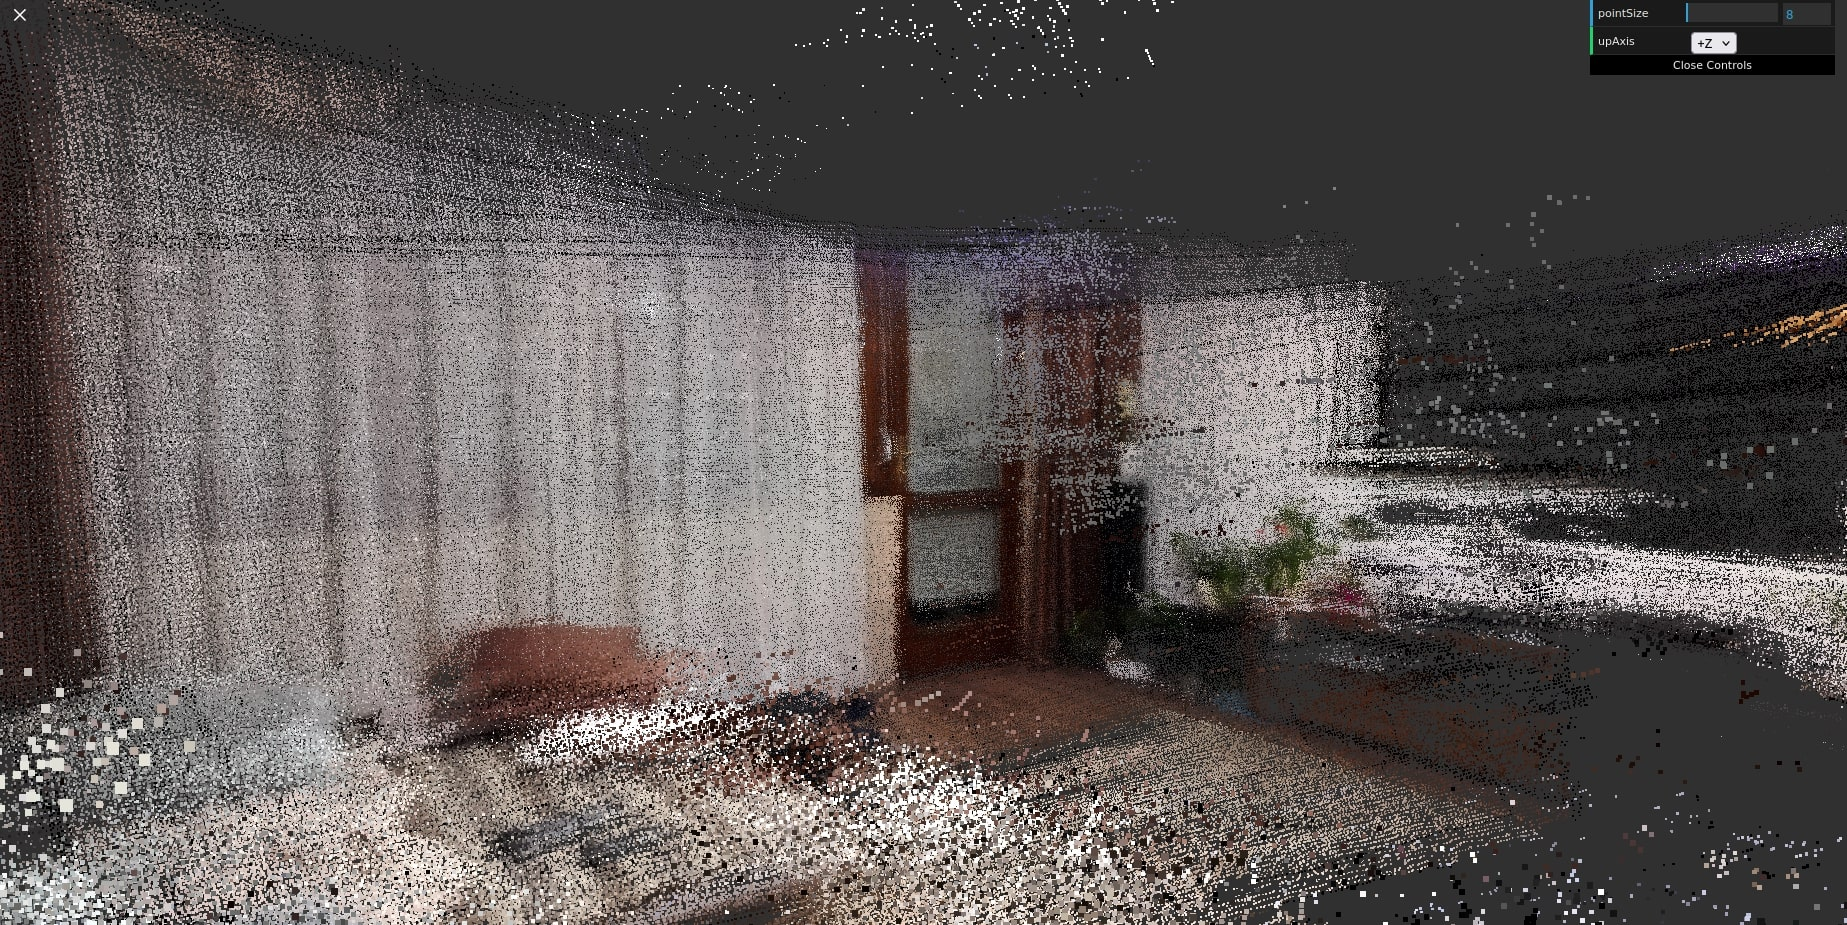
\includegraphics[width=150mm, keepaspectratio]{figures/rtabmap_ros_home.png}
	\caption{RTAB-Map ROS generated point cloud map of our living room, camera held by hand}
	\label{fig:rtabmap_nokia}
\end{figure}

\FloatBarrier
\section{RTAB-Map iOS}

We tried the iOS version of RTAB-Map as a matter of interest and it worked more effectively than the ROS version with the OAK-D camera. I used the same iPhone 13 Pro and I got a relatively good reconstruction of my apartment, as shown on Figure~\ref{fig:luma_ai_szotyi_toy}. This app can create a mesh or a photorealistic map of our surrounding. When I generated a map it was running much smoother than the ROS version: it was not lagging at all and did not lost track even in rooms with poor light. A generated mesh map can be seen on Figure~\ref{fig:rtabmap_ios}.

\begin{figure}[htbp]
	\centering
	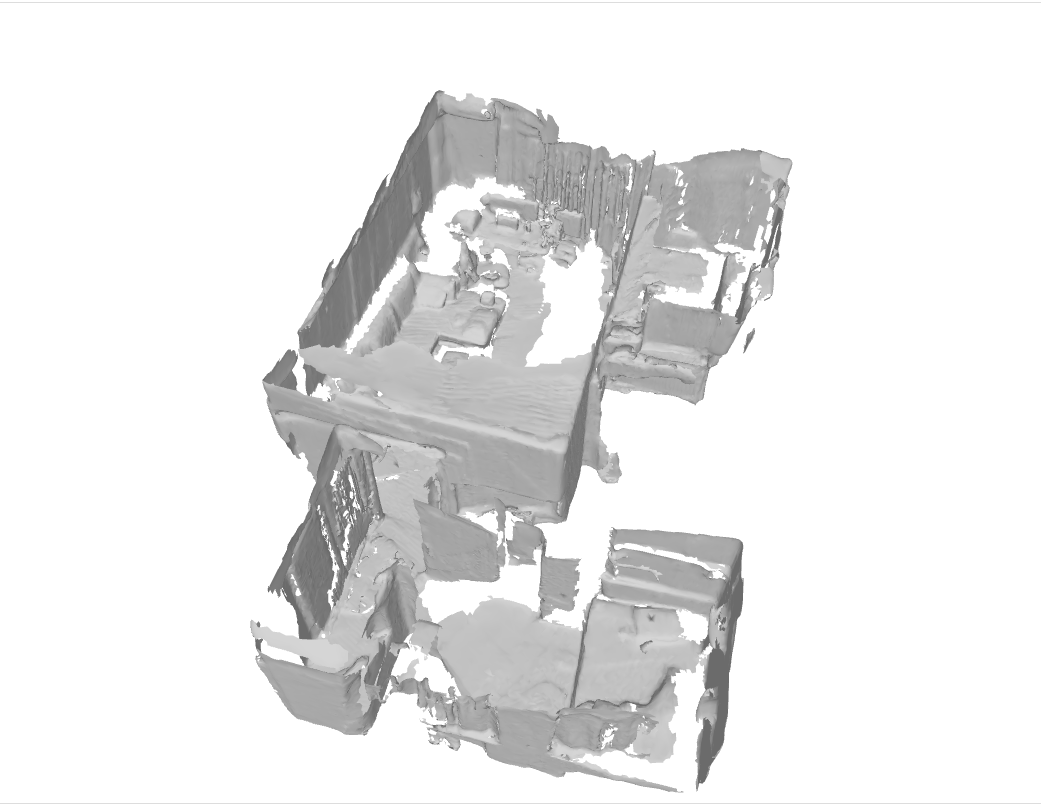
\includegraphics[width=150mm, keepaspectratio]{figures/rtabmap_ios.png}
	\caption{RTAB-Map iOS generated mesh map}
	\label{fig:rtabmap_ios}
\end{figure}

The holes in the floor are visible because the dark brown laminate reflected the light coming through the window. This made the area that RTAB-Map did not recognize due to the diversity of colors.

\section{Nvblox}

To begin using nvblox, I installed its dependencies and started the provided Docker container. However, when attempting to run the example code, I encountered frequent crashes. This was due to nvblox’s requirement for a minimum of 8 GB of VRAM, while my notebook, equipped with a GTX 1660 Ti GPU, only has 6 GB. Occasionally, the example did run successfully, as shown in Figure~\ref{fig:nvblox_example}. In this figure, you can observe how nvblox generates a voxel map by combining data from color and depth images along with LIDAR inputs, producing a comprehensive spatial map.

\begin{figure}[htbp]
	\centering
	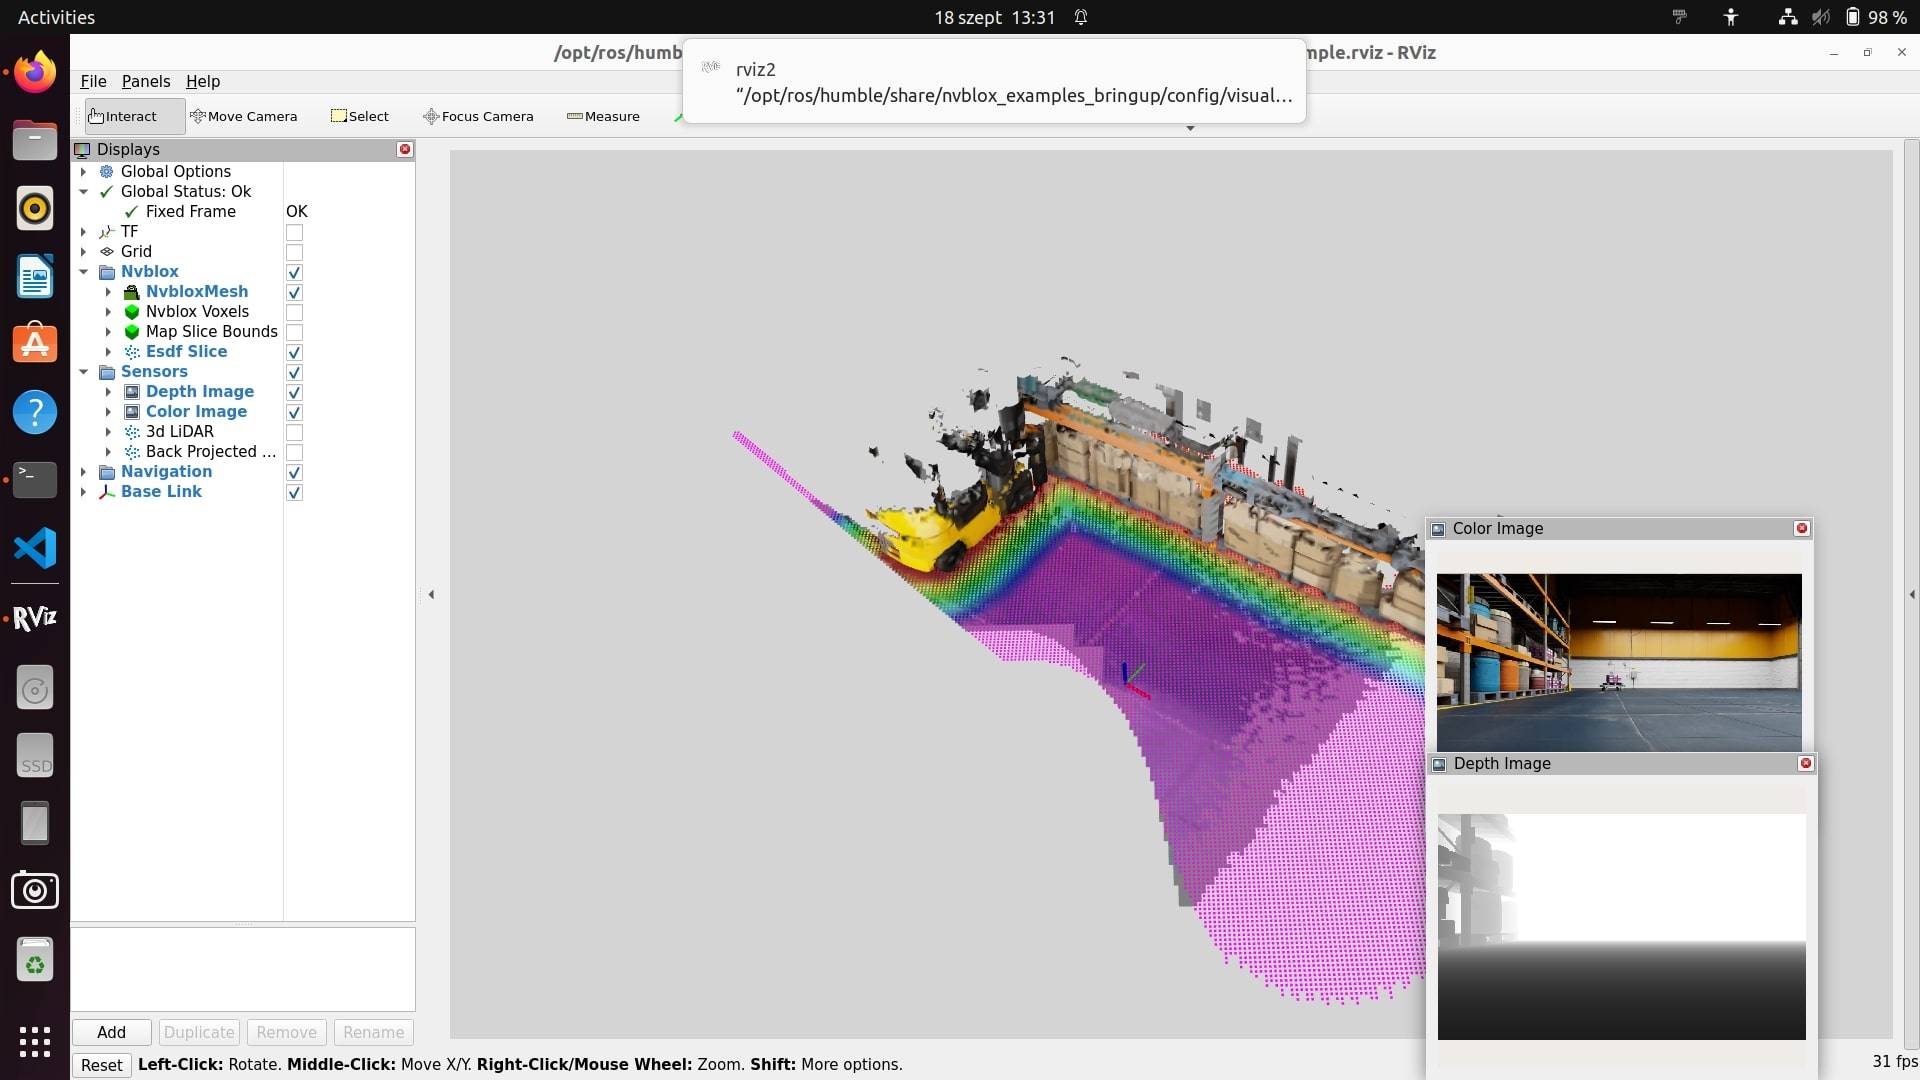
\includegraphics[width=150mm, keepaspectratio]{figures/nvblox.png}
	\caption{Running nvblox example}
	\label{fig:nvblox_example}
\end{figure}

Following my experiments with nvblox, I explored NVIDIA's Isaac VSLAM, an advanced SLAM tool that leverages NVIDIA GPUs to perform stereo visual inertial odometry (SVIO). We anticipated that Isaac VSLAM would be beneficial because it aligns well with the capabilities of the OAK-D cameras, which also support SVIO. Isaac VSLAM outputs data that can be combined with wheel odometry and LIDAR inputs, producing highly accurate localization data for ROS2's Nav2 navigation framework. Figure~\ref{fig:isaac_vslam_example} shows the Isaac VSLAM example in action. To test the Isaac VSLAM module, I used NVIDIA's isaac-sim Omniverse simulator \cite{isaac_sim_docs}. Unfortunately, the simulation environment failed to render visuals because Omniverse requires an RTX GPU to handle its advanced rendering features, which my GTX GPU could not support.

\begin{figure}[htbp]
	\centering
	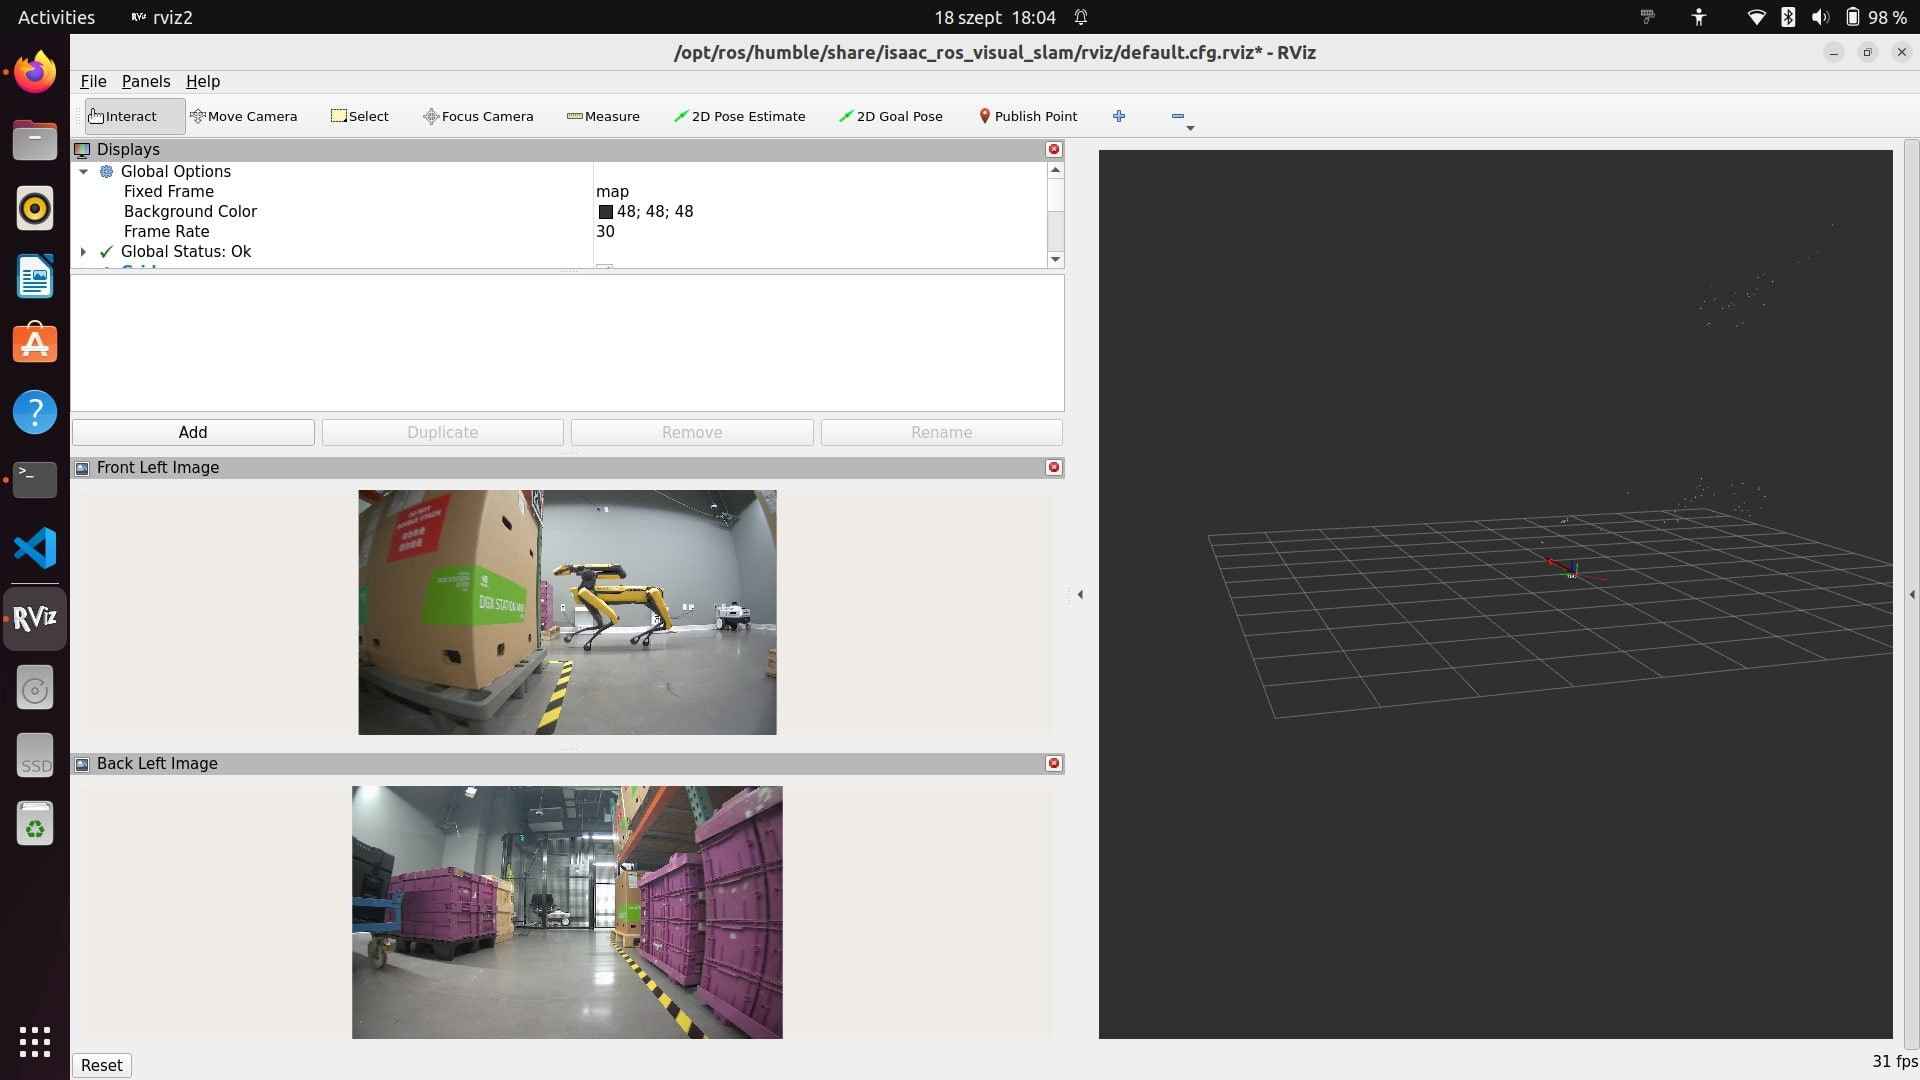
\includegraphics[width=150mm, keepaspectratio]{figures/isaac_vslam_example.png}
	\caption{Running Isaac VSLAM example}
	\label{fig:isaac_vslam_example}
\end{figure}

In the end, we opted not to use NVIDIA Isaac on the Turtlebot4 robot due to its GPU-intensive algorithms, which require at least an 8 GB VRAM-equipped Jetson module. Our robot was equipped with a Raspberry Pi 4, and we decided against investing in a Jetson due to the additional cost, which we deemed impractical for this project.
